% !TEX program = xelatex
\documentclass[aspectratio=169,11pt]{beamer}
\usepackage{fontspec}
\usepackage{xeCJK}
\usepackage{tikz}
\usepackage{booktabs}
\usepackage{tabularx}
\usepackage{array}
\usepackage{hyperref}
\usetheme[progressbar=frametitle,numbering=fraction]{metropolis}
\usetikzlibrary{arrows.meta,positioning,calc}

\setmainfont{Arial}
\setsansfont{Arial}
\setCJKmainfont{Malgun Gothic}
\setCJKsansfont{Malgun Gothic}
\setCJKmonofont{Malgun Gothic}
\xeCJKsetup{CJKspace=true}
\XeTeXlinebreaklocale "ko"
\XeTeXlinebreakskip=0pt plus 1pt
\renewcommand{\familydefault}{\sfdefault}

\definecolor{navy}{HTML}{172E3A}
\definecolor{orange}{HTML}{C95C32}
\definecolor{teal}{HTML}{087C83}
\definecolor{gold}{HTML}{9A7600}
\definecolor{whiteish}{HTML}{F4F7F8}
\definecolor{muted}{HTML}{52636D}
\definecolor{rulecolor}{HTML}{D6E0E4}
\definecolor{panel}{HTML}{F2F6F7}
\definecolor{paneldeep}{HTML}{172E3A}

\setbeamertemplate{navigation symbols}{}
\setbeamercolor{background canvas}{bg=white}
\setbeamercolor{normal text}{fg=navy,bg=white}
\setbeamercolor{frametitle}{fg=navy,bg=white}
\setbeamercolor{structure}{fg=teal}
\setbeamercolor{progress bar}{fg=teal,bg=rulecolor}
\setbeamercolor{title separator}{fg=orange}
\setbeamercolor{block title}{fg=navy,bg=white}
\setbeamercolor{itemize item}{fg=orange}
\setbeamercolor{itemize subitem}{fg=gold}
\setbeamerfont{frametitle}{series=\bfseries,size=\Large}
\setbeamerfont{normal text}{size=\small}
\setbeamersize{text margin left=0.85cm,text margin right=0.75cm}
\setlength{\parskip}{0.25em}
\newcommand{\tealtext}[1]{{\color{teal}\bfseries #1}}
\newcommand{\warn}[1]{{\color{orange}\bfseries #1}}
\newcommand{\code}[1]{{\color{navy}\ttfamily\scriptsize\detokenize{#1}}}
\newcommand{\cmdpanel}[2]{%
  {\color{#1}\bfseries #2}\par\vspace{0.12cm}
  \colorbox{paneldeep}{\parbox{0.97\linewidth}{\vspace{0.12cm}\hspace{0.12cm}\code{#2}\vspace{0.12cm}}}\par\vspace{0.2cm}}
\tikzset{box/.style={draw=rulecolor,rounded corners=0pt,fill=panel,text=navy,align=center,minimum height=0.8cm,inner sep=5pt}, arrow/.style={-{Stealth[length=2.4mm]},draw=teal,line width=1pt}}

\begin{document}

% 1
\begin{frame}[plain]
\vspace{0.78cm}
{\scriptsize\bfseries\color{teal}SOCS  /  AS/RS}\par\vspace{0.40cm}
{\huge\bfseries\color{navy}두 포크 Crane으로\par 오더 피킹 성능을 개선할 수 있을까?}\par\vspace{0.30cm}
{\large\color{muted}ACO 탐색  +  DEVS 실행 모델  +  동일 속도 조건 비교}\par\vspace{0.45cm}

\begin{tikzpicture}[x=1cm,y=1cm]
  \draw[rulecolor,line width=2pt] (0,0) -- (10,0);
  \draw[teal,line width=3pt] (4.0,0.12)--(4.0,1.55);
  \draw[gold,line width=3pt] (5.0,0.12)--(5.0,1.55);
  \fill[orange,rounded corners=2pt] (3.55,0.06) rectangle (5.45,0.52);
  \node[teal,above] at (4.0,1.55) {Fork2};
  \node[gold,above] at (5.0,1.55) {Fork1};
\end{tikzpicture}\par\vspace{0.20cm}
{\normalsize\color{muted}한 대의 Crane  $\cdot$  공유 X/Z  $\cdot$  독립 Fork1/Fork2}\par
\end{frame}

% 2
\begin{frame}{같은 인스턴스에서 두 픽업 방식을 비교}
\begin{columns}[T,onlytextwidth]
\column{0.32\textwidth}
{\color{teal}\bfseries 문제 인스턴스}\par\vspace{0.15cm}
15 $\times$ 6 rack = 90 cells\par
무작위 위치 제품 50개\par
초기 주문 10개, 총 요청 55개
\column{0.32\textwidth}
{\color{orange}\bfseries ACO 조건}\par\vspace{0.15cm}
Seeds 11, 42, 73\par
12 ants, 100 iterations\par
$\lambda=100$, makespan 목적함수
\column{0.32\textwidth}
{\color{gold}\bfseries 픽업 선택}\par\vspace{0.15cm}
Single: 한 셀, 한 제품\par
Double-capable: 가능한 인접 셀 쌍을 선택 가능\par
쌍 픽업은 같은 레벨·같은 Order
\end{columns}
\vspace{0.25cm}
\begin{center}\small\color{teal}\bfseries 목적함수 우선순위\end{center}
\begin{center}\large\bfseries 완전 주문 수\quad$\rightarrow$\quad 미출고 수량 $\times\lambda$\quad$\rightarrow$\quad makespan\end{center}
\vspace{0.2cm}
\small\color{muted}초기 재고와 주문은 동일한 저장 인스턴스를 사용합니다. ACO가 경로를 다시 찾으므로 seed별 일정은 달라집니다.
\end{frame}

% 3
\begin{frame}{포크 간격으로 인접한 두 셀을 동시에 집는다}
\begin{columns}[T,onlytextwidth]
\column{0.68\textwidth}
\begin{tikzpicture}[x=1cm,y=1cm]
  \node[box,minimum width=3.7cm,minimum height=1.35cm] (c1) at (2.2,2.3) {Cell 1\\$x=1.5$};
  \node[box,minimum width=3.7cm,minimum height=1.35cm] (c2) at (6.4,2.3) {Cell 2\\$x=2.5$};
  \draw[rulecolor,line width=3pt] (0.5,0.95)--(8.1,0.95);
  \fill[orange,rounded corners=2pt] (3.65,0.72) rectangle (4.65,1.30);
  \draw[teal,line width=3pt] (2.2,1.3)--(2.2,1.68);
  \draw[gold,line width=3pt] (6.4,1.3)--(6.4,1.68);
  \node[teal,below] at (2.2,0.60) {Fork2};
  \node[gold,below] at (6.4,0.60) {Fork1};
  \draw[arrow] (2.2,1.7)--(2.2,2.0);
  \draw[arrow] (6.4,1.7)--(6.4,2.0);
  \node[orange,below] at (4.15,0.12) {공유 rail 정지점 $x=2.0$};
\end{tikzpicture}
\column{0.30\textwidth}
\tealtext{공유 축}\par X rail, Z hoist\par\vspace{0.3cm}
\tealtext{독립 축}\par Fork1/2 reach, lift, load\par\vspace{0.3cm}
\small 두 셀 중심 간격과 포크 간격이 맞는 쌍만 동시 픽업 후보입니다.
\end{columns}
\end{frame}

% 4
\begin{frame}{픽업부터 하역까지 Crane 동작}
\begin{center}
\begin{tikzpicture}
  \node[align=center,text width=2.1cm] (a) at (0,0) {\textcolor{teal}{\bfseries 1. X/Z 이동}\\대상 셀 위치};
  \node[align=center,text width=2.1cm] (b) at (2.8,0) {\textcolor{teal}{\bfseries 2. Fork reach}\\셀 쪽으로};
  \node[align=center,text width=2.1cm] (c) at (5.6,0) {\textcolor{teal}{\bfseries 3. Box attach}\\셀에서 Crane으로};
  \node[align=center,text width=2.1cm] (d) at (8.4,0) {\textcolor{teal}{\bfseries 4. Lift / withdraw}\\포크 복귀};
  \node[align=center,text width=2.1cm] (e) at (11.2,0) {\textcolor{teal}{\bfseries 5. Unload}\\제품 전달};
  \draw[arrow] (a)--(b);\draw[arrow] (b)--(c);\draw[arrow] (c)--(d);\draw[arrow] (d)--(e);
\end{tikzpicture}
\end{center}
\vspace{0.35cm}
\begin{columns}[T,onlytextwidth]
\column{0.38\textwidth}
\tealtext{축별 속도 프로파일}\par
가속 $\rightarrow$ 정속(가능한 거리일 때) $\rightarrow$ 감속. 짧은 이동은 삼각형 프로파일이 됩니다.
\column{0.58\textwidth}
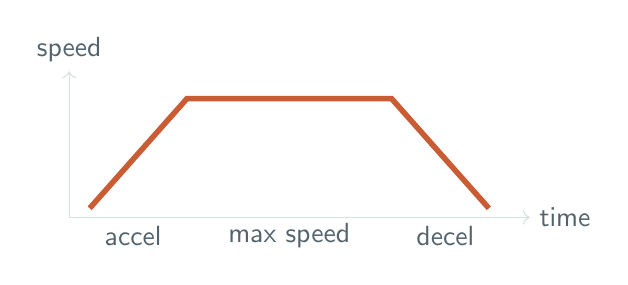
\begin{tikzpicture}[x=0.65cm,y=0.58cm]
  \draw[->,rulecolor] (0,0)--(9,0) node[right,color=muted]{time};
  \draw[->,rulecolor] (0,0)--(0,3.2) node[above,color=muted]{speed};
  \draw[orange,line width=2pt] (0.4,0.2)--(2.3,2.6)--(6.3,2.6)--(8.2,0.2);
  \node[muted] at (1.25,-0.4) {accel};\node[muted] at (4.3,-0.4) {max speed};\node[muted] at (7.35,-0.4) {decel};
\end{tikzpicture}
\end{columns}
\end{frame}

% 5
\begin{frame}{Cells, Controller, TwoForkCrane의 DEVS coupling}
\begin{center}
\begin{tikzpicture}[node distance=1.05cm and 1.2cm]
  \node[box,minimum width=3.0cm,minimum height=1.2cm] (cells) {Cells $\times$ 90\\Passive atomic models\\초기 점유 상태};
  \node[box,minimum width=3.2cm,minimum height=1.35cm,right=of cells] (ctrl) {Controller\\초기 상태 대기\\작업 배정 / idle 대기};
  \node[box,minimum width=3.1cm,minimum height=1.2cm,right=of ctrl] (crane) {TwoForkCrane\\X/Z 공유 운동\\Fork1/2 독립 동작};
  \draw[arrow] (cells.east) -- node[above,color=muted]{status} (ctrl.west);
  \draw[arrow] (ctrl.east) -- node[above,color=muted]{command} (crane.west);
  \draw[arrow] (crane.south) -- ++(0,-0.75) -| node[pos=0.25,below,color=muted]{idle / box out} (ctrl.south);
  \draw[arrow] (ctrl.south) -- ++(0,-1.25) -| node[pos=0.25,below,color=muted]{retrieve request / box transfer} (cells.south);
\end{tikzpicture}
\end{center}
\vspace{0.45cm}
\small\color{muted}Controller는 Cell과 Crane의 초기 상태를 받은 뒤 주문 작업을 배정합니다. Cell은 요청된 상자를 Crane으로 전달하고, Crane은 하역 완료 후 idle 상태를 알립니다.
\end{frame}

% 6
\begin{frame}{ACO는 단일 픽업과 가능한 쌍 픽업을 탐색}
\begin{columns}[T,onlytextwidth]
\column{0.47\textwidth}
{\color{teal}\bfseries 단일 후보}\par\vspace{0.2cm}
제품 하나의 셀을 선택\par
Fork1로 이동해 픽업\par
기존 주문별 제품 할당과 L/R 선택을 적용
\column{0.47\textwidth}
{\color{gold}\bfseries 쌍 후보}\par\vspace{0.2cm}
같은 Order 제품 2개\par
인접 bay + 같은 level일 때 허용\par
왼쪽 셀은 Fork2, 오른쪽 셀은 Fork1
\end{columns}
\vspace{0.5cm}
\begin{center}\large\bfseries 공유 X/Z 이동 + 동시 Fork 접근 + 한 번의 station 이동\end{center}
\vspace{0.3cm}
\small\color{muted}Double-capable은 두 포크가 매번 반드시 함께 집는다는 뜻이 아닙니다. ACO가 목적함수에 따라 single 또는 pair action을 고릅니다.
\end{frame}

% 7
\begin{frame}{동일 속도 조건의 실제 DEVS 비교}
\small\color{teal}\bfseries 평균 실제 coupled-DEVS makespan (simulation time units)\par\vspace{0.3cm}
\centering
\renewcommand{\arraystretch}{1.12}
\begin{tabular}{lrrrr}
\toprule
Seed & ASRS Single & 2Fork Single & 2Fork Double-capable & Paired pickups\\
\midrule
11 & 772.883 & 845.346 & \textcolor{teal}{547.775} & 18\\
42 & 778.883 & 831.346 & \textcolor{teal}{573.689} & 17\\
73 & 774.883 & 843.346 & \textcolor{teal}{539.115} & 19\\
\midrule
\textbf{Mean} & \textbf{775.550} & \textbf{840.013} & \textbf{553.526} & ---\\
\bottomrule
\end{tabular}
\vspace{0.10cm}
\begin{flushleft}\scriptsize
\textbf{속도 한계:} X/Z/Fork 최대속도 2.0, 가속·감속 1.0.\\
동일 demo.json, makespan, $\lambda=100$, ants 12, iterations 100. 각 경우 8/10 완전, 50/55 출고, 부족 5개.\\
Double-capable은 ACO가 가능한 쌍을 선택하며 전부 쌍 픽업으로 강제하지 않습니다.
\end{flushleft}
\end{frame}

% 8
\begin{frame}{속도는 같지만 단일 Crane 동작 주기는 다르다}
\begin{columns}[T,onlytextwidth]
\column{0.32\textwidth}
{\color{teal}\bfseries 기존 ASRS Single}\par\vspace{0.15cm}
{\LARGE 775.550}\par 평균 actual makespan
\column{0.32\textwidth}
{\color{orange}\bfseries 2Fork Single}\par\vspace{0.15cm}
{\LARGE 840.013}\par +8.3\% vs 기존 ASRS
\column{0.32\textwidth}
{\color{gold}\bfseries 2Fork Double-capable}\par\vspace{0.15cm}
{\LARGE 553.526}\par $-$28.6\% vs 기존 ASRS
\end{columns}
\vspace{0.4cm}
\tealtext{맞춘 조건:} 각 축의 최대속도와 가속·감속 한계.\par
\tealtext{남은 기구 차이:} 기존 Crane은 하역 뒤 Y축을 unload reach에 둡니다. 새 Crane은 Fork reach를 홈으로 retract하고, Fork1은 셀 중심에서 0.5 pitch offset입니다.\par
\small 같은 seed 42의 기존 픽업 일정을 새 Crane에서 재생해도 기존 778.883, 새 Crane 838.346이었습니다. 남은 차이는 일정 선택만으로 설명되지 않습니다.\par
\vspace{0.15cm}\warn{기존 ACO 추정치(약 304--310)는 상수 속도 모델입니다. 2Fork 보정 추정치와 직접 비교하지 말고 actual coupled-DEVS makespan을 비교합니다.}
\end{frame}

% 9
\begin{frame}{하드웨어 조건을 맞춘 비교 재현}
\tiny\color{teal}\bfseries 공통 조건: demo.json $\cdot$ makespan $\cdot$ $\lambda=100$ $\cdot$ 12 ants $\cdot$ 100 iterations $\cdot$ seeds 11 / 42 / 73\par\vspace{0.12cm}
{\color{teal}\bfseries 기존 ASRS $\cdot$ Single}\par\vspace{0.04cm}
\code{python -m examples.ASRS.run_aco_animation}\\
\code{--instance examples/ASRS/instances/demo.json --objective makespan}\\
\code{--penalty-weight 100 --seed 42 --ants 12 --iterations 100}\par\vspace{0.12cm}
{\color{orange}\bfseries ASRS\_2ForkCrane $\cdot$ Single}\par\vspace{0.04cm}
\code{python -m examples.ASRS_2ForkCrane.run_aco_animation}\\
\code{--instance examples/ASRS/instances/demo.json --objective makespan}\\
\code{--penalty-weight 100 --seed 42 --ants 12 --iterations 100 --picking-mode single --headless}\par\vspace{0.12cm}
{\color{gold}\bfseries ASRS\_2ForkCrane $\cdot$ Double-capable}\par\vspace{0.04cm}
\code{python -m examples.ASRS_2ForkCrane.run_aco_animation}\\
\code{--instance examples/ASRS/instances/demo.json --objective makespan}\\
\code{--penalty-weight 100 --seed 42 --ants 12 --iterations 100 --picking-mode double --headless}\par\vspace{0.08cm}
\tiny\color{muted}각 seed를 바꿔 반복합니다. 기존 ASRS에는 --headless가 없어 Viewer가 열립니다. 2Fork의 --headless는 coupled DEVS만 실행합니다.
\end{frame}

% 10
\begin{frame}{ACO가 결정하는 운용 항목}
\footnotesize
\renewcommand{\arraystretch}{1.24}
\begin{tabularx}{\linewidth}{>{\color{orange}\bfseries}c>{\color{gold}\bfseries}p{2.8cm}X}
1 & 주문 처리 순서 & 다음에 처리할 Order를 고릅니다.\\
2 & 제품과 셀 선택 & 요구 SKU를 채울 제품과 출고 셀을 고릅니다.\\
3 & 하역 스테이션 & 각 Order를 L 또는 R로 보냅니다. first-pickup / whole-order 정책을 적용합니다.\\
4 & 묶음과 방문 순서 & 방문 순서와 인접 제품의 두 포크 동시 픽업 여부를 정합니다.
\end{tabularx}
\vspace{0.45cm}
\small\color{muted}현재 single 모드는 픽업 묶음에서 단일 제품만 허용합니다.
\end{frame}

% 11
\begin{frame}{2포크 피킹: 현재 구현과 확장 선택지}
{\color{teal}\bfseries 현재 구현}\par\vspace{0.15cm}
\textbf{Single pick}\quad 한 셀로 이동 $\rightarrow$ 한 포크로 픽업 $\rightarrow$ L/R 하역\par\vspace{0.12cm}
\textbf{Double mode}\quad 인접한 두 셀, 같은 레벨에 정렬 $\rightarrow$ 두 포크 동시 픽업 $\rightarrow$ L/R 하역\par
\small\color{muted}현재 double은 같은 Order의 인접 셀 제품을 한 정지점에서 함께 픽업합니다.\par\vspace{0.35cm}
{\color{gold}\bfseries 확장 가능한 연속 픽업}\par\vspace{0.15cm}
\begin{center}\large 첫 셀 픽업 $\rightarrow$ 다른 셀로 이동 $\rightarrow$ 두 번째 픽업 $\rightarrow$ L/R 하역\end{center}
두 번째 제품은 같은 Order 또는 다른 Order에서 선택할 수 있습니다. 다른 Order까지 함께 운반하려면 두 Order의 하역 스테이션 호환성도 결정해야 합니다.\par\vspace{0.2cm}
\warn{연속 픽업과 여러 Order를 한 운반에 묶는 방식은 현재 구현에 포함되지 않습니다.}
\end{frame}

\end{document}

